\documentclass[preview]{standalone}

\usepackage{amsmath}
\usepackage{amssymb}
\usepackage{stellar}
\usepackage{bettelini}
\usepackage{wrapfig}

\hypersetup{
    colorlinks=true,
    linkcolor=black,
    urlcolor=blue,
    pdftitle={Biologia},
    pdfpagemode=FullScreen,
}

\begin{document}

\id{biologia-sistema-nervoso}
\genpage

\section{Il sistema nervoso}

\begin{snippetdefinition}{sistema-nervoso-definition}{Sistema nervoso}
    Il \textit{sistema nervoso} permette la trasmissione di segnali tra le diverse parti dell'organismo e
    la coordinazione delle sue funzioni volontarie e involontarie. È formato dal sistema nervoso
    centrale (SNC) e dal sistema nervoso periferico (SNP).
\end{snippetdefinition}

\begin{snippetdefinition}{sistema-nervoso-centrale-definition}{Sistema nervoso centrale}
    Il \textit{sistema nervoso centrale} è costituito dall'encefalo e dal midollo spinale.
    La sua funzione è quella di ricevere e analizzare le informazioni in
    arrivo dall'ambiente interno ed esterno dell'organismo e di elaborare le risposte più appropriate.
\end{snippetdefinition}

\begin{snippetdefinition}{sistema-nervoso-periferico-definition}{Sistema nervoso periferico}
    Il \textit{sistema nervoso periferico} è costituito dai 
    gangli e dai nervi, che collegano il sistema nervoso centrale
    con le varie parti del corpo.
    La sua funzione è dunque quella di mandare input e output.
\end{snippetdefinition}

\begin{snippet}{nervous-sys-illustration}
    \setlength{\intextsep}{0pt}%
    \begin{wrapfigure}{l}{0.7\textwidth}
        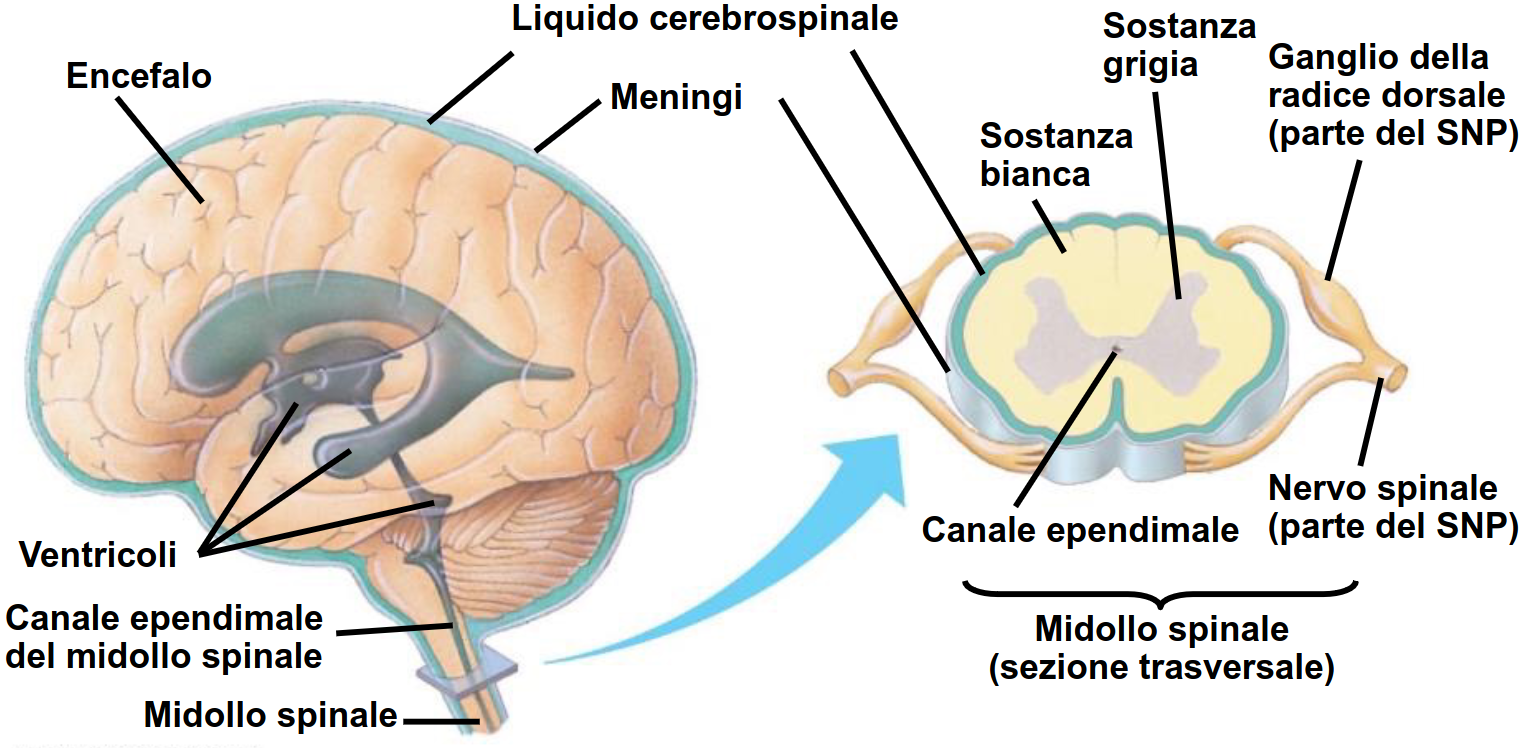
\includegraphics[width=0.7\textwidth]{./resources/nervous_system.png}
        \caption{Sistema Nervoso}
        \vspace{-1cm}
    \end{wrapfigure}
    
    Le funzioni del sistema nervoso sono le seguenti:
    \begin{enumerate}
        \item \textbf{ricezione} dell'input sensoriale dai recettori sensoriali;
        \item \textbf{integrazione}, ovvero interpretazione dei segnali sensoriali ed elaborazione di risposte;
        \item \textbf{emissione} dell'output motorio, ovvero trasmissione dei segnali alle cellule effettrici.
    \end{enumerate}
    
    \wrapfill
\end{snippet}

\section{Neurone}

\begin{snippetdefinition}{dendride-definition}{Dendride}
    I \textit{dendriti} sono dei prolungamenti ramificati che
    permettono al neurone di captare gli stimoli provenienti da altri
    neuroni.
\end{snippetdefinition}

\begin{snippetdefinition}{corpo-cellulare-definition}{Corpo cellulare}
    Il \textit{corpo cellulare} è una struttura che contiene
    il nucleo e gli altri organuli cellulari.
\end{snippetdefinition}

\begin{snippetdefinition}{cono-derivazione-definition}{Cono di derivazione assonica o di emergenza}
    Il \textit{cono di derivazione assonica} o \textit{di emergenza}    
    è il segmento iniziale dell'assone che integra le informazioni
    raccolte dai dendriti e avvia i potenziali d'azione.
\end{snippetdefinition}

\begin{snippetdefinition}{assone-definition}{Assone}
    L'\textit{assone} è il prolungamento che permette il passaggio del
    potenziale d'azione dal corpo cellulare fino
    alle terminazioni sinaptiche, in prossimità delle cellule bersaglio.
\end{snippetdefinition}

\begin{snippetdefinition}{terminazione-sinaptica-definition}{Terminazione sinaptica o terminale d'assone}
    La \textit{terminazione sinaptica} o \textit{terminale d'assone}
    consiste in ramificazioni del neurone che permettono
    la comunicazione con più cellule.
\end{snippetdefinition}

\begin{snippetdefinition}{bottone-sinaptico-definition}{Bottone sinaptico}
    Il \textit{bottone sinaptico} è la parte terminale del neurone,
    ossia il punto di passaggio dell'informazione da un neurone
    alla cellula successiva, che può essere una cellula nervosa,
    muscolare o endocrina.
\end{snippetdefinition}

\begin{snippet}{neuron-illustration}
    \setlength{\intextsep}{0pt}%
    \begin{wrapfigure}{r}{0.4\textwidth}
        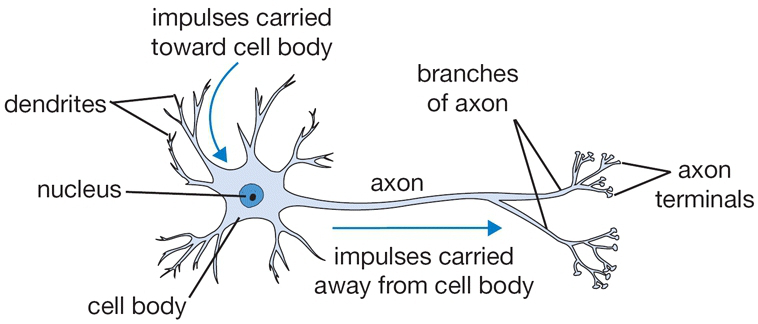
\includegraphics[width=0.35\textwidth]{./resources/neuron.png}
        \caption{Neurone}
        \vspace{-1cm}
    \end{wrapfigure}

    Le funzioni delle parti di un neurone sono:
    \begin{itemize}
        \item \textbf{dendriti e parte del corpo cellulare:} ricezione dei segnali;
        \item \textbf{cono di emergenza:} integrazione;
        \item \textbf{assone:} conduzione del segnale elettrico;
        \item \textbf{terminazioni dell'assone:} trasferimento del segnale ad altre cellule.
    \end{itemize}

    Possiamo distinguere le seguenti categorie di cellule:
    \begin{enumerate}
        \item \textbf{cellule presinaptiche:} neurone che trasmette l'informazione;
        \item\textbf{cellule postsinaptica:} cellula nervosa, muscolare o endocrina che riceve il segnale.
    \end{enumerate}

    \wrapfill
\end{snippet}

\begin{snippetdefinition}{neurone-sensoriale-definition}{Neuroni sensoriali o afferenti}
    I \textit{neuroni sensoriali} o \textit{afferenti} sono
    cellule nervose con funzione di conduzione. Le terminazioni dendritiche di questi neuroni
    sono associate ai recettori sensoriali e trasportano informazioni sotto forma di segnale
    elettrico, dai recettori esterni e interni ai neuroni del SNC.
\end{snippetdefinition}

\begin{snippetdefinition}{neurone-interconnessione-definition}{Neuroni di interconnessione o interneuroni}
    I \textit{neuroni di interconnessione} o \textit{interneuroni} sono
    cellule nervose del SNC che hanno la funzione di ricevere messaggi nervosi che
    provengono dai neuroni afferenti, per trasmetterli, attraverso molteplici connessioni, ad altri
    neuroni del SNC che li integrano ed elaborano.
\end{snippetdefinition}

\begin{snippetdefinition}{neurone-motori-definition}{Neuroni motori o efferenti}
    I \textit{neuroni motori} o \textit{efferenti} sono
    cellule nervose che hanno la funzione di condurre la risposta allo stimolo, elaborata nel
    SNC, agli organi effettori.
\end{snippetdefinition}

\begin{snippet}{categorie-nervi}
    Possiamo distinguere le seguenti categorie di nervi:
    \begin{enumerate}
        \item \textbf{nervi sensoriali:} trasportano segnali afferenti;
        \item \textbf{nervi motori:} trasportano segnali efferenti;
        \item \textbf{nervi misti:} trasportano segnali afferenti ed efferenti.
    \end{enumerate}
\end{snippet}

\begin{snippetdefinition}{gangli-definition}{Gangli}
    I \textit{gangli} sono piccole masse
    costituite dall'aggregazione dei corpi cellulari dei neuroni del SNP.
\end{snippetdefinition}

\begin{snippetdefinition}{nuclei-definition}{Nuclei}
    I \textit{nuclei} sono piccole masse
    dall'aggregazione dei corpi cellulari dei neuroni del SNC.
\end{snippetdefinition}

\begin{snippet}{tipi-cellile-neuronali}
    Le cellule del sistema nervoso che non sono neuroni si chiamano cellule \textit{gliali}.
    Esse sono più abbondanti dei neuroni e hanno svariate funzioni.
    Vi sono le cellule
    \begin{itemize}
        \item \textbf{di Schwann:} producono una sostanza isolante (mielina) che isola l'assone nel sistema nervoso periferico;
        \item \textbf{oligodendrociti:} producono una sostanza isolante (mielina) che isola l'assone nel sistema nervoso centrale.
    \end{itemize}
\end{snippet}

\begin{snippetdefinition}{sinapsi-definition}{Sinapsi}
    La \textit{sinapsi} è il posto dove si scambia l'informazione
    fra il neurone pre sinaptico e post sinaptico.
\end{snippetdefinition}

\begin{snippet}{differenza-potenziale-neuroni}
    La differenza di potenziale nelle cellule dei neuroni è di -70 mV. Ogni cellula è caricata
    negativamente data la minoranza di cariche positive al suo interno.
    Tenere una differenza di potenzia necessita quindi ATP.
\end{snippet}

\section{Ventricoli, sostanza grigia e sostanza bianca nel SNC dei vertebrati}

\begin{snippet}{midollo-expl}
    Il midollo possiede una zona interna più scura (zona grigia), e una zona esterna più chiara
    (zona bianca). Nella zone grigia abbiamo la maggior parte dei corpi cellulari,
    mentre nella zona bianca abbiamo gli assoni.

    L'effettore è quella parte che corpo che risponde allo stimolo.

    Nel midollo ci sono risposte brevi e i segnali vengono elaborati solo minimamente per determinare se devono passare o meno.
    Tutte le elaborazioni complesse vengono effettuate dall'encefalo.

    Il sodio cerca di entrare perché c'è né di meno all'interno, ma ce ne sarà di meno perché appena entra
    viene buttato fuori dalla pompa.
    Al contrario, il potassio cerca di uscire e la pompa lo ributta sempre all'interno.

    % domanda esame: tutte le celle in ordine fra un segnale rosso che si vede in TV o il dito che cambia canale
\end{snippet}

\end{document}